\chapter{Background}
\label{C:background}

\section{Neural Networks and Deep Learning}

Since Krizhevsky et al.'s AlexNet \cite{alexnet} in 2012, many problems are increasingly being solved best by Artificial Neural Networks (NN). Any particular NN is not designed but discovered by gradient descent, where the parameters of the NN are iteratively improved with respect to a loss function, and a dataset.

Many variants exist, and in this section I firstly introduce and clarify my notation, and then give an overview of the different aspects of neural networks to contextualize my work.

\subsection{Notation}
\label{ss:dl-notation}

Since we are often using tensors of rank 3 or higher in neural network implementations, it is useful to have some notation that clarifies how functions are applied across these dimensions.

First, a simple example using activation functions. The ReLU activation function is defined as:
\begin{align}
\label{eqn:relu}
\begin{aligned}
    \fdef{\relu}{\R}{\R} \\
    \relu&(x) ≝ \max(0,x)
\end{aligned}
\end{align}
It is customary to use the symbol $\phi$ for activation functions. Activation functions are typicall scalar functions, but are applied independently across all components of a tensor. To represent such, I will use the following notation, for example, applying the ReLU activation function to a vector $\x$:
\begin{equation*}
\x'_i = \relu(\x_i)
\end{equation*}
In the above equation, the subscript $i$ shows that the function is applied \textit{independently} to each component of the vector $\x$.

This notation also works for multiple dimensions, including when an operation is not applied independently across some dimension. For example, the following is how I will show the \textit{softmax} function, which is a vector valued function, applied independently across the rows of a $B\times N$ matrix $\X$ (which is used in the definition of the attention operation in \Cref{C:transformers}).

The softmax function is defined as:
\begin{equation}
\label{eqn:softmax}
\begin{split}
    \nvfdef{\sigma}{N}{N} \\
    \sigma(\x_n) ≝ \frac{e^{\x_{n}}}{\sum_{n'} e^{\x_{n'}}}
\end{split}
\end{equation}
We can apply the the above function to a matrix $\X \in \R^{B\times N}$ independently over $B$ as follows:
\begin{align*}
\X'_{b,n} &= \sigma(\X_b)_{n} \\
          &= \frac{e^{\X_{b,n}}}{\sum_{n'} e^{\X_{b,n'}}}
\end{align*}

The term $\X_b$ refers to the $b$-th row of $X$ as a vector, as is common in tensor algebra software such as NumPy \cite{numpy} or TensorFlow \cite{tensorflow}. Here however the order of the subscript indices $b$ and $n$ is ignored -- the indices index their respectively-named dimensions. This that we abandon the distinction between row- and column-vectors. I will thus be explicit when applying matrix and vector products.

I will now define some simple neural networks as examples for clarifying any later notation.

I will typically use $N$ for the input dimensionality of a network, and $D$ for the \textit{embedding} (or \textit{hidden} / \textit{latent}) dimensionality.  Let $\x \in \R^{N}$ be some input data embedded into an $N$-dimensional vector space. Let $W \in \R^{N \times D} $ be a matrix of learned weights, and let $\phi \colon \R \to \R$ be some non-linear function. Then, the computation done by one layer of a simple fully-connected neural network is represented as follows.
\begin{align}
\label{eqn:mlp}
\begin{aligned}
    f&_{\text{mlp}} \colon \R^N \to \R^D \\
    f&_{\text{mlp}}(\x) ≝ \phi(W\x) + \boldsymbol{b}
\end{aligned}
\end{align}
\begin{gather*}
    W \in \R^{N \times D}, \quad \vb \in \R^D
\end{gather*}
$W$ is the weight matrix, and $\vb$ is the bias vector, which together are the parameter set for this simple model. The output of the neural network is a $D$-dimensional vector.

A simple classifier network would be defined as follows, for $N$ dimensional data classified into $C$ classes, with $L$ hidden layers:
\begin{align}
\label{eqn:classifier}
\begin{aligned}
    \vfdef{f_0}{N}{D} \\
    f_{0}&(\x) = \phi(W_0 \x) + \vb &
    W_0 &\in \R^{N\times D} &
    \vb_0 &\in \R^{D}
\\ \\%
    \vfdef{f_\l}{D}{D} & \forall \l &\in 1,\dots,L \quad \\
    f_\l&(\x) = \phi(W_\l f_{\l-1}(\x)) + \vb_\l &
    W_\l &\in \R^{D\times D} \quad &
    \vb_\l &\in \R^{D}
\\ \\%
    \vfdef{f_L}{D}{C} \\
    f_{L}&(\x) = \sigma(W_L f_{L-1}(\x) + \vb_L) &
    W_L &\in \R^{D \times C} &
    \vb_L &\in \R^{C}
\\ \\%
    \vfdef{f_{\text{classifier}}}{N}{C} \\
    f_{\text{classifier}}& = f_L \circ f_{L-1} \circ \cdots \circ f_0 &
    \theta &= \rlap{\{$W_0, \cdots, W_L, \vb_0, \cdots, \vb_L \} $}
\end{aligned}
\end{align}
The parameters of the network are $\theta = \{$W0, ..., WL, vb0, ..., vbL-1$\}$. The output of the network is a $C$-dimensional vector, where each component is the probability that the input belongs to that class. This model would be trained with a categorical cross-entropy loss function -- which I will discuss in the next section.

\vspace{5cm}

\pagebreak

\subsection{Tasks}

Neural networks are applied to a wide variety of tasks, which lead to a number of different choices for the architecture and loss function. In this section, I will help to contextualize my later work by giving a brief overview of the ways that different neural networks and training setups differ.

On the following pages, I give some simple ontologies of the different considerations that combine to define a particular task and architecture, in particular:
\begin{enumerate}
    \item Training objective / loss function (\Cref{fig:ontology-loss})
    \item Data dimensionality / length (\Cref{fig:ontology-input-shape})
    \item Dataset format (\Cref{fig:ontology-task})
\end{enumerate}


\begin{figure}
    \centering
    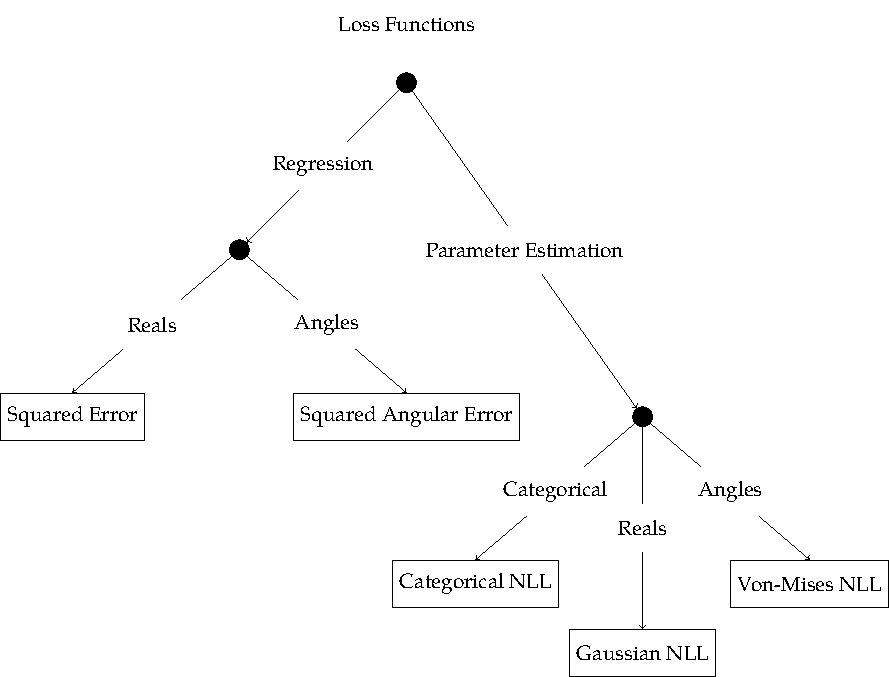
\includegraphics[]{figures/ontology-1-loss.pdf}
    \vspace{1cm}
    \captionsetup{parskip=7pt}
    \caption[Ontology of loss functions.]{We can split loss functions into two categories.

    In the former, the loss function has the form of an error function. When minimizing this function, the model learns to output the expected value of the posterior $\E\left[p(y \mid x)\right]$ of the output $y$ given the input $x$. This is called a regression or maximum-a-posteriori (MAP) task.

    In the latter, the loss function has the form of a negative-log-likelihood (NLL) function. The model outputs the parameters of a probability distribution, and the loss function is the negative log-likelihood of the data under that distribution. This includes the case of categorical NLL (also called categorical cross-entropy), where the model outputs a probability distribution over a discrete set of classes.

    Models trained with a NLL loss learn to output an explicit posterior distribution $p(y \mid x)$, given a fixed functional form for $p$, such as a Gaussian, mixture of Gaussians, Categorical, Von-Mises, etc. Depending on the task, and output format, different functional forms for $p$ may be appropriate.}
    \label{fig:ontology-loss}
\end{figure}


\begin{figure}
    \centering
    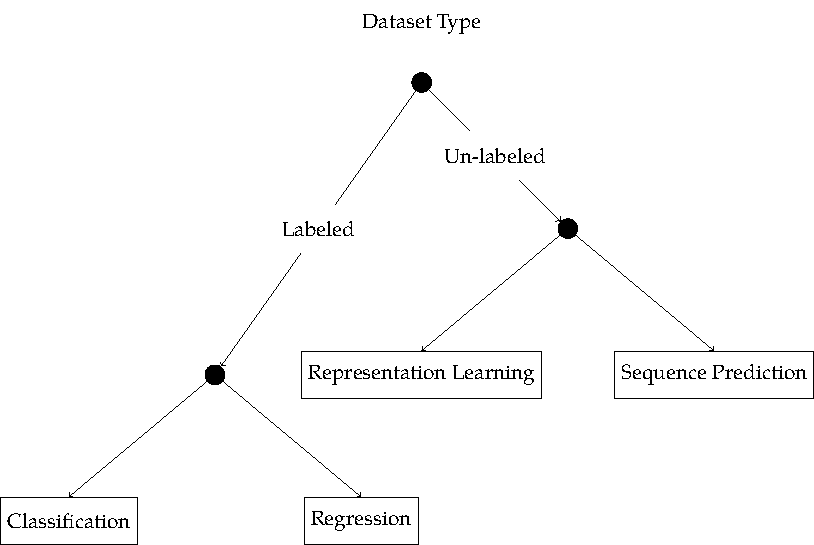
\includegraphics[]{figures/ontology-2-task.pdf}
    \vspace{1cm}
    \captionsetup{parskip=7pt}
    \caption[Ontology of dataset types]{
        Basic ontology of dataset types.

        When data is explicitly labeled a model can be trained on a task directly. However, the labeling process is often expensive, and in many cases, the data is unlabeled.

        When learning on unlabeled data, the goal is to learn a representation of the data that is useful for some downstream task.
    }
    \label{fig:ontology-task}
\end{figure}



\begin{figure}
    \centering
    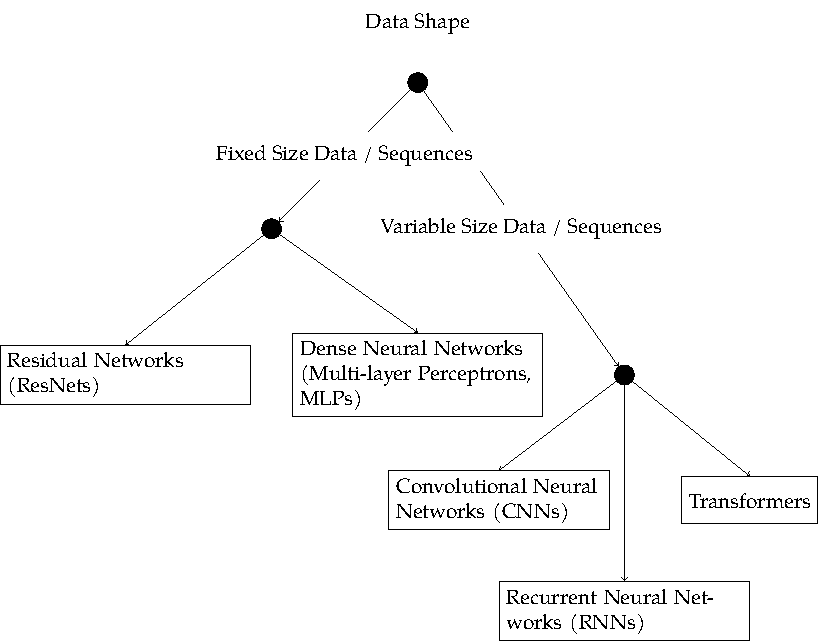
\includegraphics[]{figures/ontology-3-input-shape.pdf}
    \vspace{1cm}
    \captionsetup{parskip=7pt}
    \caption[Fixed vs variable input shape]{Neural network variants which support variable input shape.

    Due to their construction, MLPs and ResNets are restricted to a fixed input shape, and so can only be trained and used on data that is of a fixed size, such as tabular data, or data that has been processed into a fixed size by re-sampling, chunking etc.

    RNNs, CNNs and Transformers can accept variable length data, each with their own tradeoffs. They are typically more suitable for data that is naturally of variable size/length, such as text, audio or images.}
    \label{fig:ontology-input-shape}
\end{figure}


The choice of training objective affects the settings in which a model can be used, which theoretical properties we get from it, and more. The structure of the data affects the type of model that can be used, and the format of the dataset affects what tasks we can learn from it.

The simplest kind of training objective is regression. When we train a model with a regression objective it learns to predict the expected value of the output. Regression is characterized by using an error function as the loss, for example \textit{mean-squared-error}:
\newcommand{\mse}{L_{\text{MSE}}}
\begin{align}
\label{eqn:mse}
\begin{split}
    \fdef{\mse}{\R^{N×D}×\R^{N×D}}{\R} \\
    \mse&(y, \hat{y})_{ni} ≝ \frac{1}{N} \sum_n\left[ \sum_i (y_{ni} - \hat{y}_{ni})^2 \right]
\end{split}
\end{align}
This function sums the error over the \textit{feature} dimension $D$ and averages the error over the \textit{batch} dimension $N$ \footnote{Averaging has no effect on the optimization, it is simply that dividing by the batch and/or sequence length means that the loss value remains in the same range independent of the batch size or sequence length.}. Training a model by minimising this loss function, is equivalent to maximising the likelihood of a Gaussian distribution. Given input $x$, the model output $y = f(x)$ can be interpreted as $\E[p(y|x)]$.
